\section{A Debugging Scenario}\label{sec:example}

\begin{figure}[t]
  \centering
  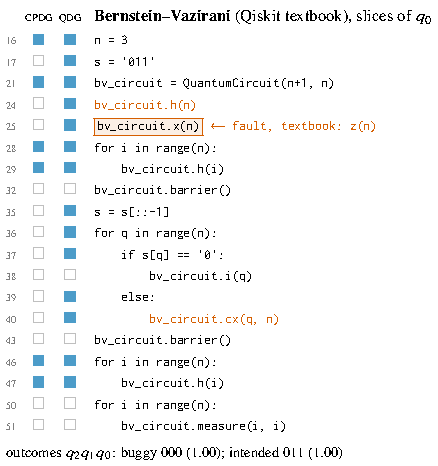
\includegraphics[width=\columnwidth]{figures/fig_bv.pdf}
  \caption{The Bernstein--Vazirani program of the Qiskit textbook~\cite{qiskittextbook}, with comments and
  blank lines omitted and the textbook's line numbers kept. Line~25 carries a seeded fault, \texttt{x(n)}
  where the textbook applies \texttt{z(n)}. The two columns mark the statements in the backward slice of
  $q_0$ under the classical PDG and under the QDG. The classical PDG misses the orange lines, which are
  dependences of $q_0$. Slices are computed by our tool statically, and outcomes and dependences by the
  study's code.}
  \label{fig:bv}
\end{figure}

The Bernstein--Vazirani algorithm~\cite{bernstein1997qct} finds a hidden bit string $s$ with a single query
to an oracle that computes the parity of $s \wedge x$. Fig.~\ref{fig:bv} shows the program of the Qiskit
textbook~\cite{qiskittextbook}, with $s = 011$. The algorithm rests on phase kickback. Lines~24 and~25
prepare the auxiliary qubit $q_3$ in $\ket{-}$, a superposition of $0$ and $1$ with opposite signs. Each
CNOT of line~40 has the auxiliary as its target, and on $\ket{-}$ it leaves the target unchanged and flips
the phase of its control instead. The Hadamard gates of line~47 turn these phases into the bits of $s$. We
seeded one fault, a one-token change on line~25 that applies $X$ instead of $Z$. The auxiliary is then left
in $\ket{+}$, on which a CNOT acts as the identity, and the program returns \numBvBuggyOut{} instead of
\numBvFixedOut{}.

The developer sees $q_0$ read $0$ where $s$ says $1$, and slices backward from $q_0$ to see which
statements determine it. A classical slicer follows data and control dependence. It reads
\texttt{cx(q, n)}, the controlled-NOT that flips its target when its control is $1$, as the assignment
$q_n \leftarrow q_n \oplus q$, which reads $q$ and writes only the auxiliary. Its slice of $q_0$ keeps the
Hadamard gates of lines~\numBvCpdgLines{} and the statements that compute their qubits, lines
\numBvCpdgClassical{}, as the left column of Fig.~\ref{fig:bv} shows. The slice even appears to be right.
Its \numBvCpdgOps{} operations give $q_0$ the same state as the whole program, with fidelity
\numBvCpdgFidelity{}, where fidelity measures the similarity of two quantum states and is $1$ exactly when
they are equal. Two Hadamard gates on $q_0$ show nothing wrong, and the slice gives the developer no
reason to look at lines~\numBvMissedLines{}, where the fault is.

These lines are nonetheless dependences of $q_0$. Restoring $Z$ on line~25 turns $q_0$ from $\ket{0}$ into
$\ket{1}$, two states with fidelity \numBvFixFidelity{}. A CNOT acts on its control as well as its target.
The QDG, in which every gate reads and writes all its qubits, keeps lines~\numBvQdgLines{}, exactly the
dependences of $q_0$, together with the statements that compute them, among them the oracle's loop and
condition on lines~35 to~39. Its slice contains the fault. Entanglement plays no part here, since $q_0$ is in
a pure state after every operation and so is never entangled with the auxiliary.

Choosing a single qubit as the criterion was enough here, because the fault shows in $q_0$ alone. It is not
always enough. In a real bug from Bugs4Q~\cite{zhao2023bugs4q}, posted on Stack Overflow, a two-qubit
program meant to prepare $(\ket{01}+\ket{10})/\sqrt{2}$ applies \texttt{h(1)} where \texttt{x(1)} was
needed, and returns all four bit strings equally often. Each qubit alone reads $1$ with probability
\numMotPOne{}, in the buggy program and in the intended one alike, and the error lies only in the
correlation between the two. A criterion that names a single qubit, as the classical criterion $(s, V)$
does when $V$ is one qubit, cannot express this failure. The criterion must be the pair $\{q_0, q_1\}$.

The two lessons scale. Reading a gate as an assignment misses influence that flows into a control qubit,
and a one-qubit criterion misses errors in correlations.
